\section{Auswertung}
\label{sec:Auswertung}
% \subsection{Fehlerrechnung}
% Der Mittelwert einer physikalischen Größe $a$ mit $N$ Einzelmesswerten ist gegeben durch
% \begin{equation}\label{eq:mean}
%     \overline{x}=\frac{1}{N}\sum_{i=1}^Na_\text{i}\,.
% \end{equation}
% Die Standardabweichung eines Mittelwerts zu einer physikalischen Größe a bestimmt sich mit
% \begin{equation}\label{eq:std}
%     \Delta{x}=\sqrt{\frac{1}{N(N-1)}\sum_{i=1}^N\left(a_\text{i}-\overline{x}\right)}\,.
% \end{equation}

% \begin{table}[H]
%   \centering
%   \caption{}
%   \label{tab:}
%   \begin{tabular}{S[table-format=2.1] S[table-format=4] S[table-format=2.1] S[table-format=4]S[table-format=3]S[table-format=2.1]}
%       \toprule
%       {}&{}&{}&{}&{}\\
%       \midrule
      
%       \bottomrule
%   \end{tabular}
% \end{table}

% \begin{figure}[H]
%   \centering
%   \includegraphics{build/}
%   \caption{.}
%   \label{fig:}
% \end{figure}

\subsection{Kalibrierung des Detektors}

Um den Germaniumdetektor zu kalibrieren wird eine $^{152}\text{Eu}$-Probe verwendet und dessen Spektrum gemessen.
Die Energie der Gamma-Quanten wird dabei aus der Literatur entnommen. 
Des Weiteren wurde eine Untergrundmessung durchgeführt und nach einer Normierung von der $^{152}\text{Eu}$-Messung abgezogen.
Die Normierung bezieht sich auf die unterschiedlichen Messzeiten von Europium- und Untergrundmessung.
Das Spektrum der Untergrundstrahlung ist in Abbildung \ref{fig:untergrund} dargestellt.

\begin{figure}[H]
  \centering
  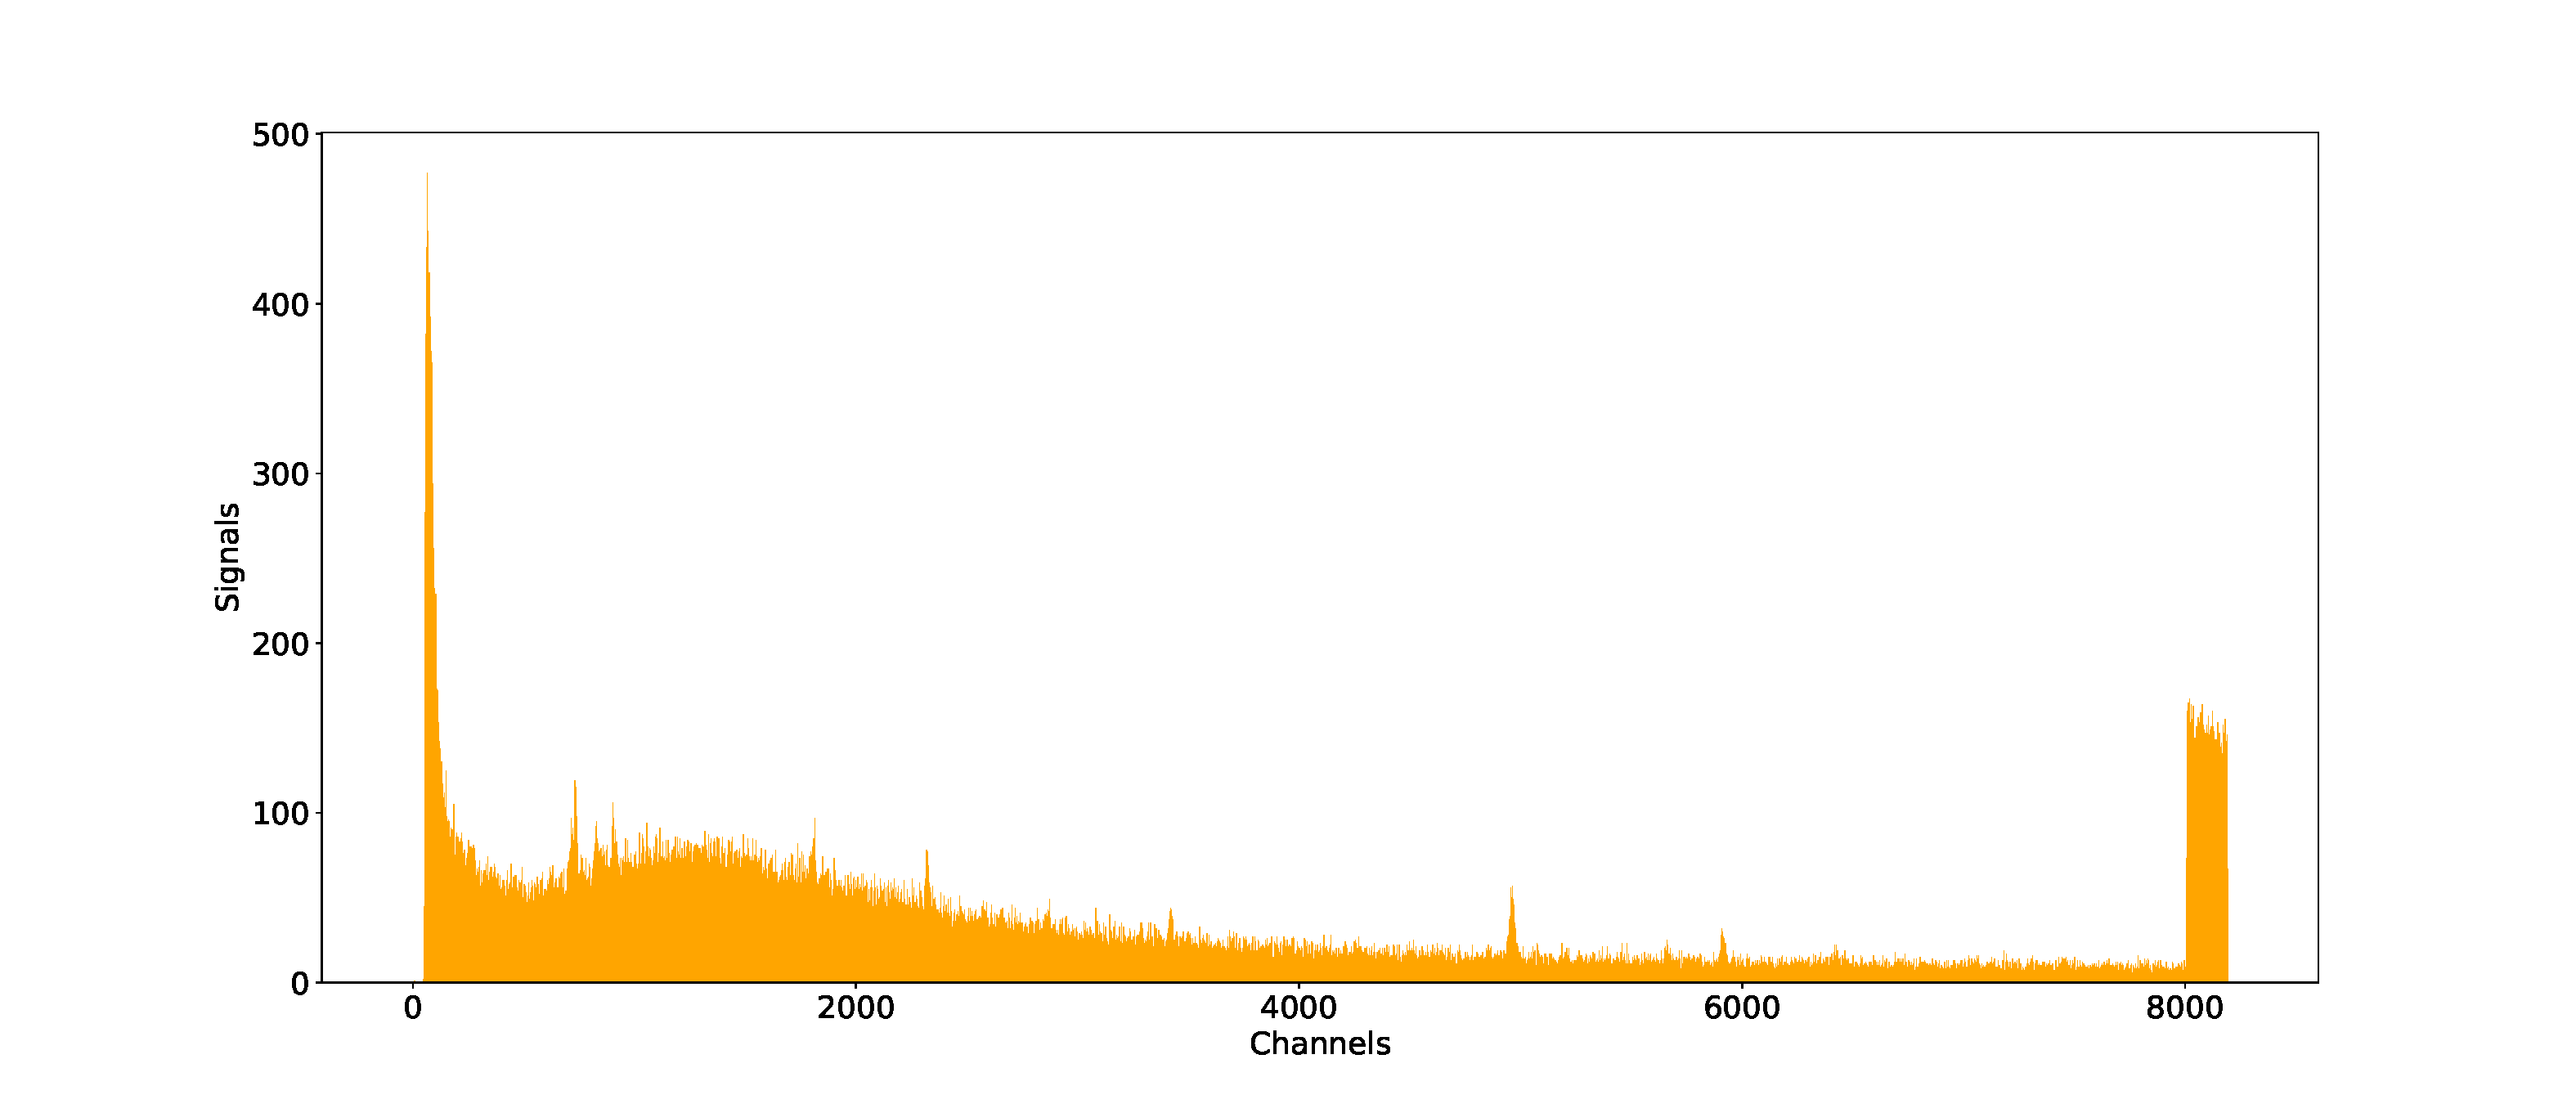
\includegraphics[width=\textwidth]{../plots/Untergrund.pdf}
  \caption{Spektrum der Untergrundstrahlung.}
  \label{fig:untergrund}
\end{figure}

Um den Kanälen des Detektors eine Energie zuzuordnen, wurden zunächst die prominentesten Peaks des $^{152}\text{Eu}$-Spektrums identifiziert 
und mit den wahrscheinlichsten Emissionsenergien aus der Literatur verglichen.
Die Peaks wurden mit Hilfe von \texttt{find\_peaks} der python-Bibliothek \texttt{scipy} \cite{scipy} 
identifiziert.
Die Peaks und die zugehörigen Energien sind in Tabelle \ref{tab:eu} aufgeführt und in Abbildung \ref{fig:eu} dargestellt.

\begin{figure}[H]
  \centering
  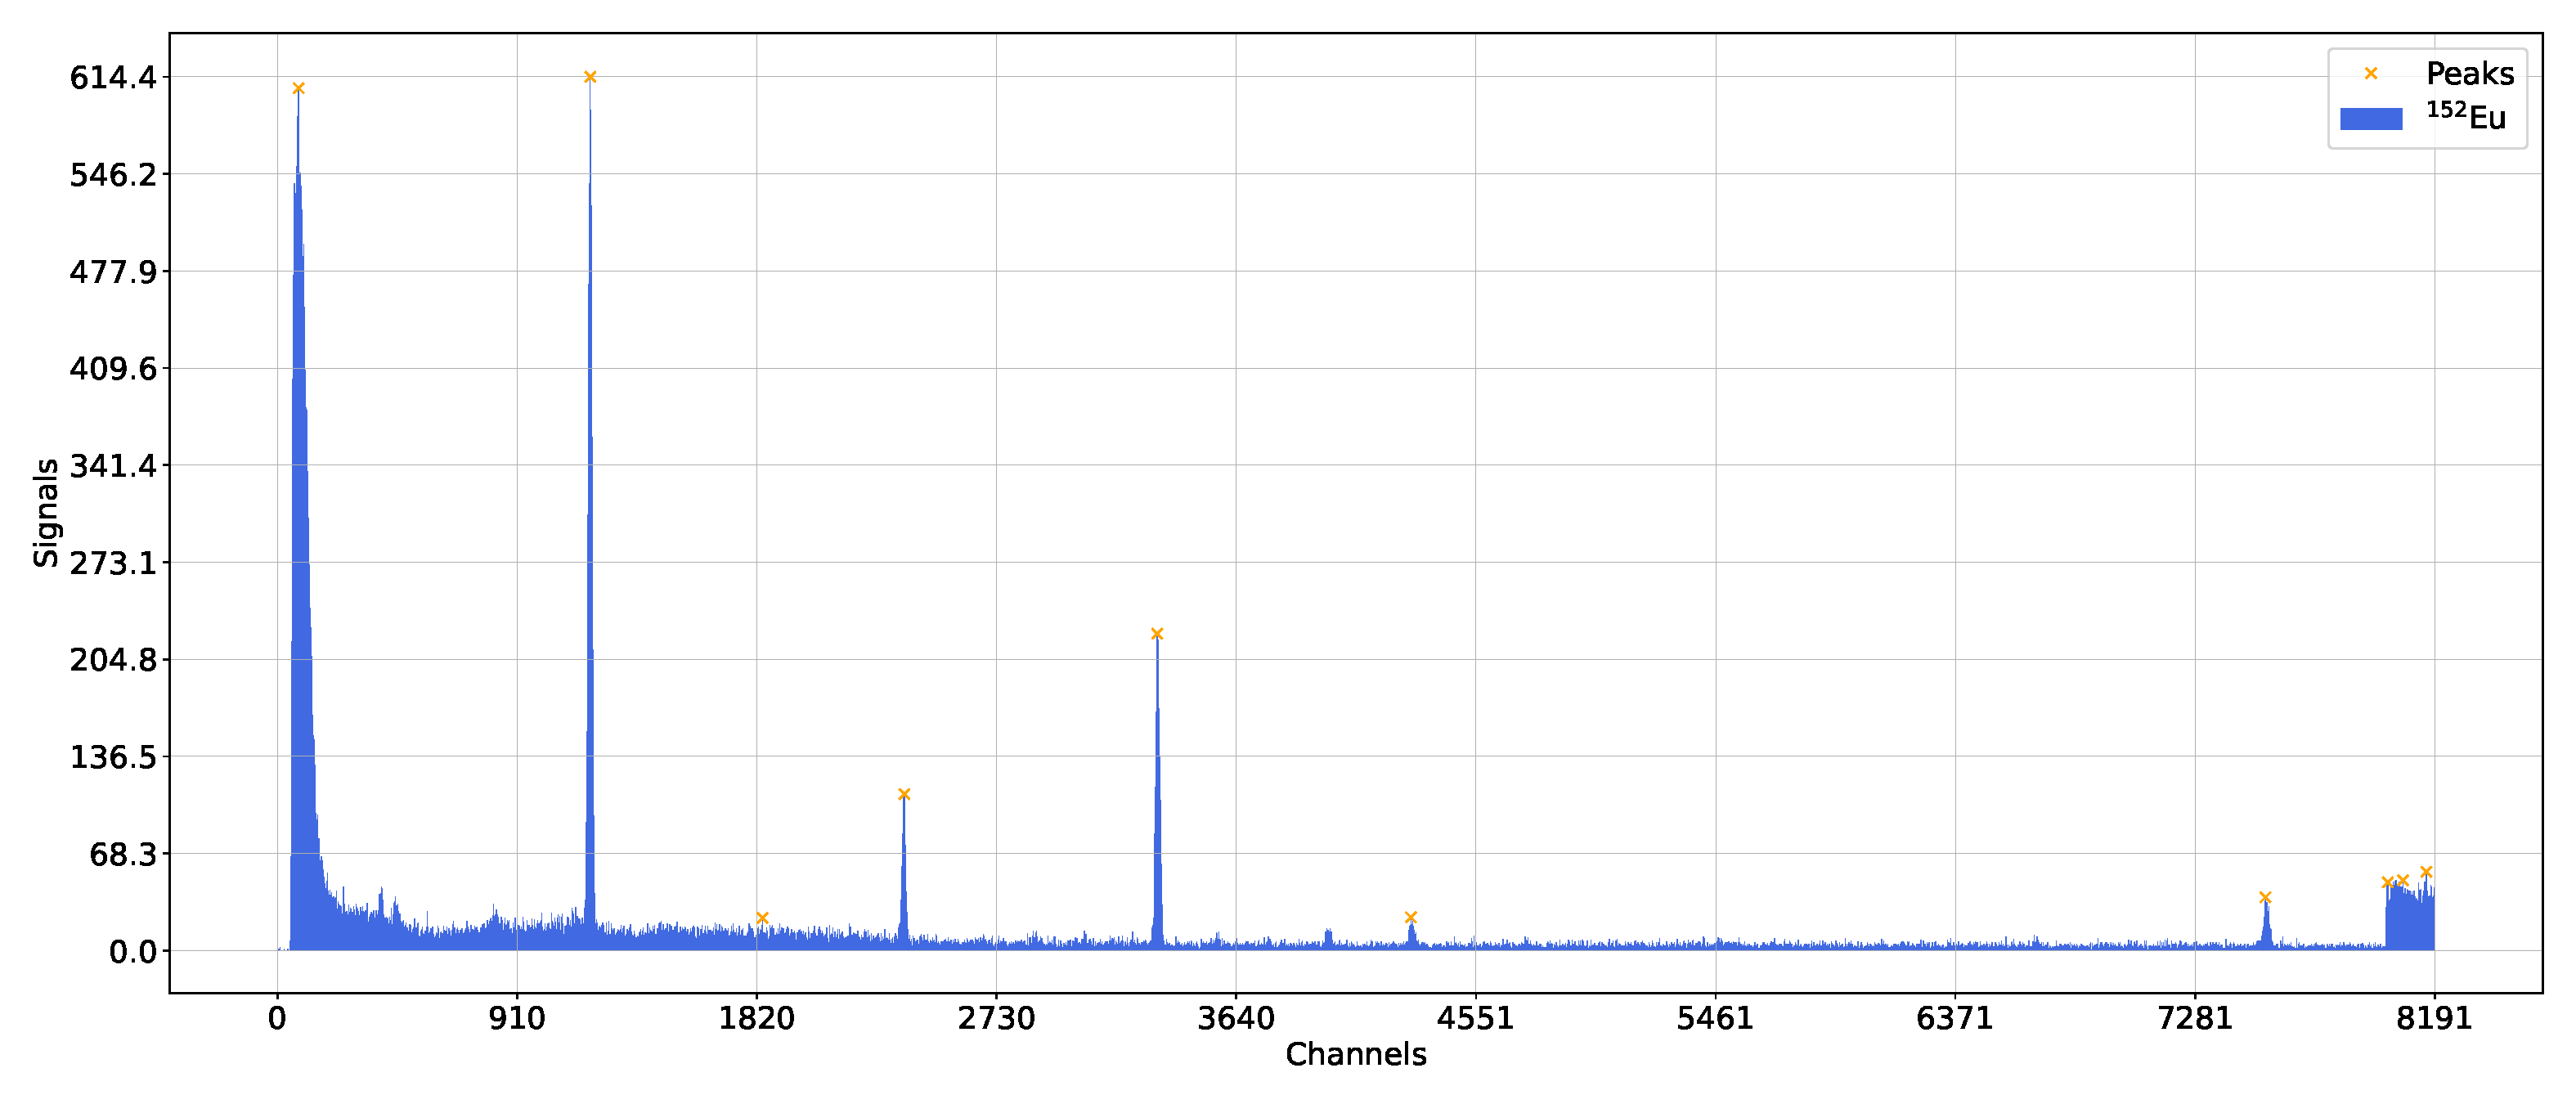
\includegraphics[width=\textwidth]{../plots/Europium-Peaks.pdf}
  \caption{Spektrum der $^{152}\text{Eu}$-Probe und dessen prominentesten Peaks.}
  \label{fig:eu}
\end{figure}

\begin{table}[H]
  \centering
  \caption{Energien und Wahrscheinlichkeiten der Vollenergiepeaks der $^{152}\text{Eu}$-Probe sowie die zugenorndeten Kanäle.}
  \label{tab:eu}
  \begin{tabular}{S S[table-format=4] S[table-format=3.1] S}
      \toprule {$E_\text{Lit} / \si{\kilo\electronvolt}$} & {$P_\text{Lit} /\si{\percent}$} & {Kanal} & {Counts}\\
      \midrule
      121.7817& {28.41 \pm 0.13}&1187&{10159.0 \pm 222}\\
      344.2785& {26.59 \pm 0.12}&2380&{1806.1	\pm 83} \\
      778.9045& {12.97 \pm 0.06}&3340&{3771.6 \pm 189} \\
      964.079 & {14.5 \pm 0.06} &3985&{269.6 \pm	50} \\
      1112.076& {13.41 \pm 0.06}&4303&{388.6 \pm	34} \\
      1408.013& {20.85 \pm 0.08}&7548&{686.1 \pm	80} \\
      \bottomrule
  \end{tabular}
\end{table}

Die Kalibrierung erfolgt durch eine lineare Regression der Form

\begin{equation}
  E = a \cdot K + b
\end{equation}

und stellt damit eine Beziehung zwischen Kanalnummer $K$ und Energie $E$ her.
Die Parameter der Regression betragen

\begin{align*}
    a = {0.228334 \pm 0.0} \, \si{\kilo\electronvolt} \\
    b = -148.659709 \pm 0.000593 \, \si{\kilo\electronvolt} \, 
\end{align*}

und werden im weiteren Verlauf zur Energiebestimmung der Peaks verwendet.
Der Fit ist in Abbildung \ref{fig:kalibrierung} dargestellt.

\begin{figure}[H]
  \centering
  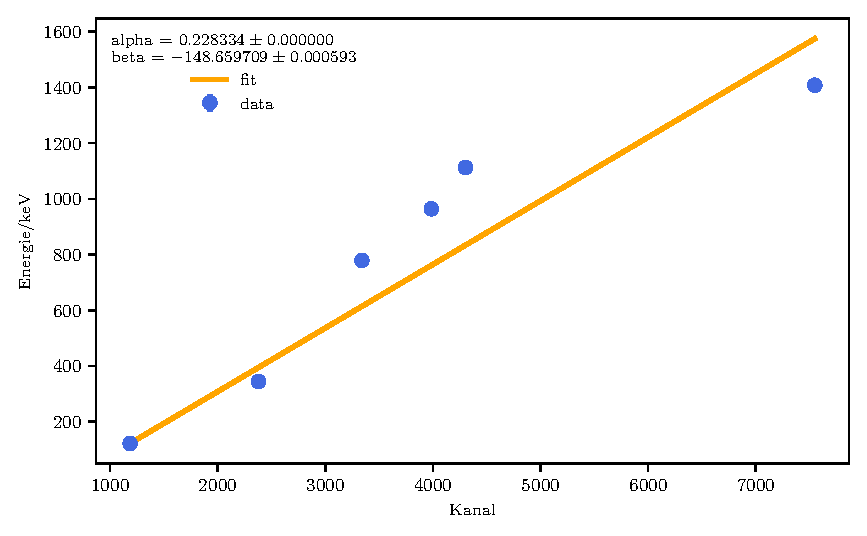
\includegraphics[width=\textwidth]{../plots/Europium-Fit.pdf}
  \caption{Ausgleichsfunktion der gemessenen Energien und der zugeordneten Kanäle.}
  \label{fig:kalibrierung}
\end{figure}

\subsection{Vollenergie-Detectionswahrscheinlichkeit}
Die Vollenergie-Detectionswahrscheinlichkeit $Q$ ist durch 
\begin{equation}
  Q = \frac{4 \pi N}{\Omega A P t}
\end{equation}
gegeben.
Dabei ist $N$ die Anzahl der gemessenen Photonen, $\Omega$ der Raumwinkel, $A$ die Aktivität, $P$ die Emissionswahrscheinlichkeit und $t$ die Messzeit.
Die Werte für die Emissionswahrscheinlichkeit und die Anzahl der gemessenen Photonen sind in Tabelle \ref{tab:eu} aufgeführt.
Der Raumwinkel des Germaniumdetektors beträgt
\begin{equation}
  \frac{\Omega}{4\pi} =\frac{1}{2}\left(1-\frac{a}{\sqrt{a^2+r^2}}\right) 
\end{equation}
mit den Werten 
\begin{align*}
  a &= 2.25 \, \si{\centi\meter} \\
  r &= 8.52 \, \si{\centi\meter} \, .
\end{align*}
Somit ergibt sich ein Raumwinkel von $\Omega = 0.01657$.
Die Aktivität der $^{152}\text{Eu}$-Probe betrug am Tag der Produktion (01.10.2000) $A_0 = (4130 \pm 60) \, \si{\becquerel}$.
Die Aktivität $A$ zum Messzeitpunkt wird durch
\begin{equation}
  A = A_0 \cdot \exp\left(-\frac{\ln(2)}{t_{1/2}} \cdot t\right)
\end{equation}
berechnet.
Mit einer Halbwertszeit von $t_{1/2} = 13.522$ Jahre ergibt sich am Tag der Messung (21.10.2024) 
eine Aktivität von $A = ( 1203 \pm 17 ) \, \si{\becquerel}$.
Die berechnete Vollenergie-Detectionswahrscheinlichkeit ist in der Tabelle \ref{tab:fedp} aufgeführt.

\begin{table}
    \centering
    \caption{Vollenergie-Detectionswahrscheinlichkeit der $^{152}\text{Eu}$-Probe.}
    \label{tab:fedp}
    \begin{tabular}{S S[table-format=1.5]}
        \toprule {$E_\text{Lit} / \si{\kilo\electronvolt}$} & {$Q / \si{\percent}$} \\
        \midrule
        121.7817&{0.06200	\pm 0.00165}\\
        344.2785&{0.01178	\pm 0.00057}\\
        778.9045&{0.05042	\pm 0.00264}\\
        964.079 &{0.00322	\pm 0.0006}\\
        1112.076&{0.00502	\pm 0.00045}\\
        1408.013&{0.00571	\pm 0.00067}\\
        \bottomrule
    \end{tabular}
\end{table}
